% !TEX TS-program = pdflatex
% !TEX encoding = UTF-8 Unicode

%************************************************
\chapter{Strumento di nuova concezione}
\label{Strumento di nuova concezione}
%************************************************

Come non cadere nel fascino della creazione tramite "tavole musicali" come avviene
in Cage o evitare di intraprendere un percorso musicale legato al teatro, dove
diventa più importante il gesto stesso che la composizione e la forma? Semplice,
tramite un'analisi specifica degli strumenti in questione.

Appena la nostra ricerca, da ammaliante, diventa analitica, allora il tutto
diventa più chiaro e si perdono anche le facili sperimentazioni sulla realtà e
si va a conoscere una bibliografia sempre più estesa e ci si perde, verso, appunto,
l'ignoto.

Reputo essenziale nella vita di un compositore di musica elettroacustica,
l'avvicinamento al mondo \textit{liuteristico} e di costruzione, semplicemente
perché il realizzare qualcosa di fisico, comporta il contatto con la materia e
la possibilità di avvicinarsi \textit{con mano} al suono che si vuole andare a
formare, o modificare e trasformare.

La scuola del compositore che immagina, scrive, e solo in seguito dà vita alle
proprie opere, a mio parere, è ormai lontana, perché sovviene un nuovo
importante aspetto legato al suono: la complessità spettrale legata alle
armoniche, alla fusione e l’evoluzione di formanti, ma soprattutto alla caduta
di un regime tonale e di armonia classica, verso \textit{micro-variazioni} e
\textit{micro-ritmiche} legate sia all’universo microscopico che a quello macroscopico.

La fisica è giunta ormai a studiare delle parti sempre più piccole della materia,
poiché proprio all’interno del più piccolo frammento di essa si può trovare la
nostra origine e delle risposte legate all’evoluzione.



%************************************************


\section{Unamolla}

Indico \textbf{Unamolla} come \textit{strumento di nuova concezione}, uno
strumento composto da "una molla" in ferro armonico, una base in legno e un
sistema di amplificazione a contatto.

% Paolo Zavagna, in alcuni suoi appunti pubblicati sul suo sito
% internet\footnote{http://www.zavagna.it/paolo/}, redige una classificazione
% degli \textit{strumenti musicali elettronici}, qui definisce gli strumenti
% \textbf{Elettromagnetici}:

Facendo riferimento alla classificazione indicata da
Zavagna\footnote{http://www.zavagna.it/paolo/}, % il link deve puntare all'articolo preciso
degli \textit{strumenti musicali elettronici}, egli così definisce gli strumenti
\textbf{Elettromagnetici}:

\begin{quotation}
Gli strumenti musicali elettromeccanici che producono il suono tramite un’azione
meccanica di riproduzione di una forma d’onda, che può essere "scritta" su un
nastro in movimento o su un disco rotante.
\end{quotation}

Unamolla è quindi, uno strumento elettromagnetico di nuova concezione.

\subsection{Passaggio da installazione a strumento}

Nel 2018, quando ideai \emph{Sp.I.R.E.} [installazione di molle e piastre regolate ed
elettrificate], notai subito che un difetto assai visibile era la trasportabilità.

Se in passato bastava scrivere una partitura e nell’eventualità trasportare il
mio personal computer, ora avevo creato un “oggetto” costruito appositamente per
tale scopo e (per quanto ci fosse un progetto alle spalle) molto cose erano
riproduzioni fisiche di schizzi creati con carta e penna. In seguito, tramite le
mie ricerche sulla performance musicale e lo sviluppo di varie tecniche per la
gestualità sullo \emph{Sp.I.R.E.}, decisi di utilizzare un oggetto sonoro per volta,
dedicandomi ad un limitato numero di parti: due. Utilizzai quindi \textit{Unamolla}
in acciaio ed una piastra in rame\footnote{le prime erano in ferro armonico e
zincato, le seconde in acciaio}; infine, decisi di dedicarmi ad un unica parte
e limitai la mia attenzione esclusivamente alla molla.

Se \emph{Sp.I.R.E.} era uno strumento composto da 4 molle e 2 piastre in grado, tramite
degli attuatori, di auto-eccitarsi, Unamolla è uno strumento meno complesso nella
costruzione, ma più complesso nel sistema di ripresa. Lo \emph{Sp.I.R.E.} aveva come
sistema di ripresa solo 4 microfoni a contatto e due microfoni posizionati ai
lati per donare una stereofonia all'ascolto. Nel caso di Unamolla, invece, la
diffusione è \textbf{mono} ed è più complessa dello \emph{Sp.I.R.E.}, perché è in realtà
una somma di più fonti di ripresa sonora collocate sullo strumento.

\begin{figure}[t]
\centering
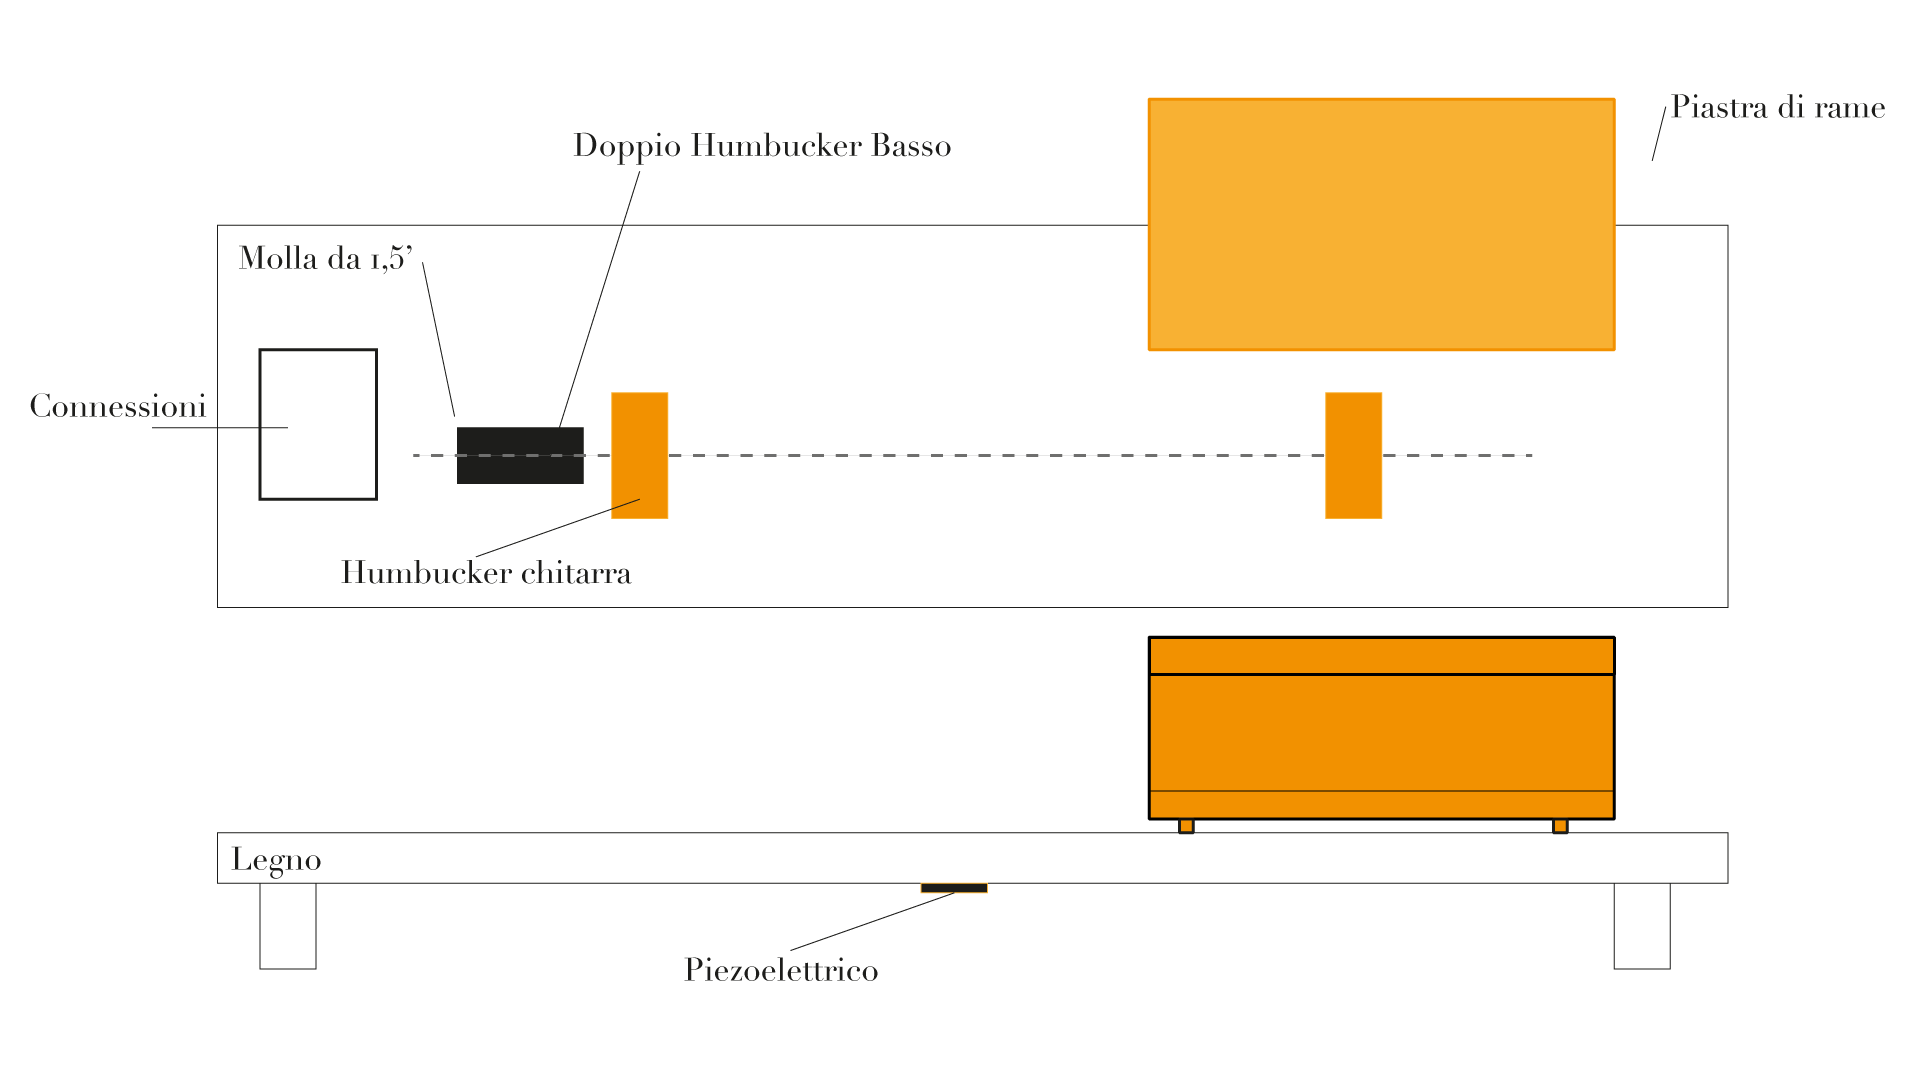
\includegraphics[width=1.\textwidth]{unamolla_schema.png}
\caption{Schema \emph{Unamolla 1.0}}
\label{fig:02_unamolla_01}
\end{figure}

\subsection{Sistema di amplificazione \textit{UNAMOLLA}}

Durante la costruzione dello \emph{Sp.I.R.E.}, avevo notato che il segnale non era
trasdotto perfettamente (utilizzavo solo dei piezoelettrici), mancava di attacco
e le dinamiche erano davvero piatte. Aggiunsi quindi su una tavola di legno,
prima uno, poi due humbucker (per chitarra e per basso) in aggiunta al
iezoelettrico e fui soddisfatto del risultato. Ho potuto, quindi, definire
\textit{Unamolla} come \textit{strumento musicale} ed iniziare la mia analisi
gestuale.

Unamolla si può definire uno strumento a \textbf{spettro inarmonico} costituito,
nel primo prototipo, da una lastra di ottone e di una molla in ferro-armonico,
connesse da una tavola di legno di noce. Questo primo prototipo, che ho chiamato:
\emph{Unamolla 1.0}, ha subìto con il tempo delle variazioni ulteriori dalla figura che
segue e, con il tempo ho diminuito ulteriormente la sua grandezza e ho diviso
piastra e molla.

In figura \ref{fig:02_unamolla_01}, lo schema di costruzione di \emph{Unamolla 1.0}.

Nello schema è disegnata la tavola di legno sulla quale è fissata una molla da
1,5 pollici e la piastra di rame, opportunamente disaccoppiata tramite una vite
inferiore al contatto con il legno e una vite superiore di fissaggio. Sul lato
sinistro della molla ho posto un doppio Humbucker per basso elettrico ed in
seguito, ho diviso, alle due estremità, i due humbucker per chitarra. Al di
sotto della parte in legno troviamo un piezoelettrico.

\emph{Unamolla 1.0} è stato il primo stadio, il primo prototipo di strumento. Anche se
le dimensioni erano estremamente diminuite, la trasportabilità dello strumento
era ancora in fase di cambiamento, dato che ogni volta dovevo smontarlo e
montarlo, ma soprattutto alcuni gesti erano difficilmente eseguibili.

Decisi quindi di lavorare su una seconda \textit{Unamolla}  e ho creato il secondo
prototipo: ho eliminato la lastra (come scritto in precedenza) per dare spazio
ad un design più consono per eseguire determinati gesti legati anche all’uso
dell’archetto.

%************************************************
\section{Analisi acustica}

\begin{figure}[t]
\centering
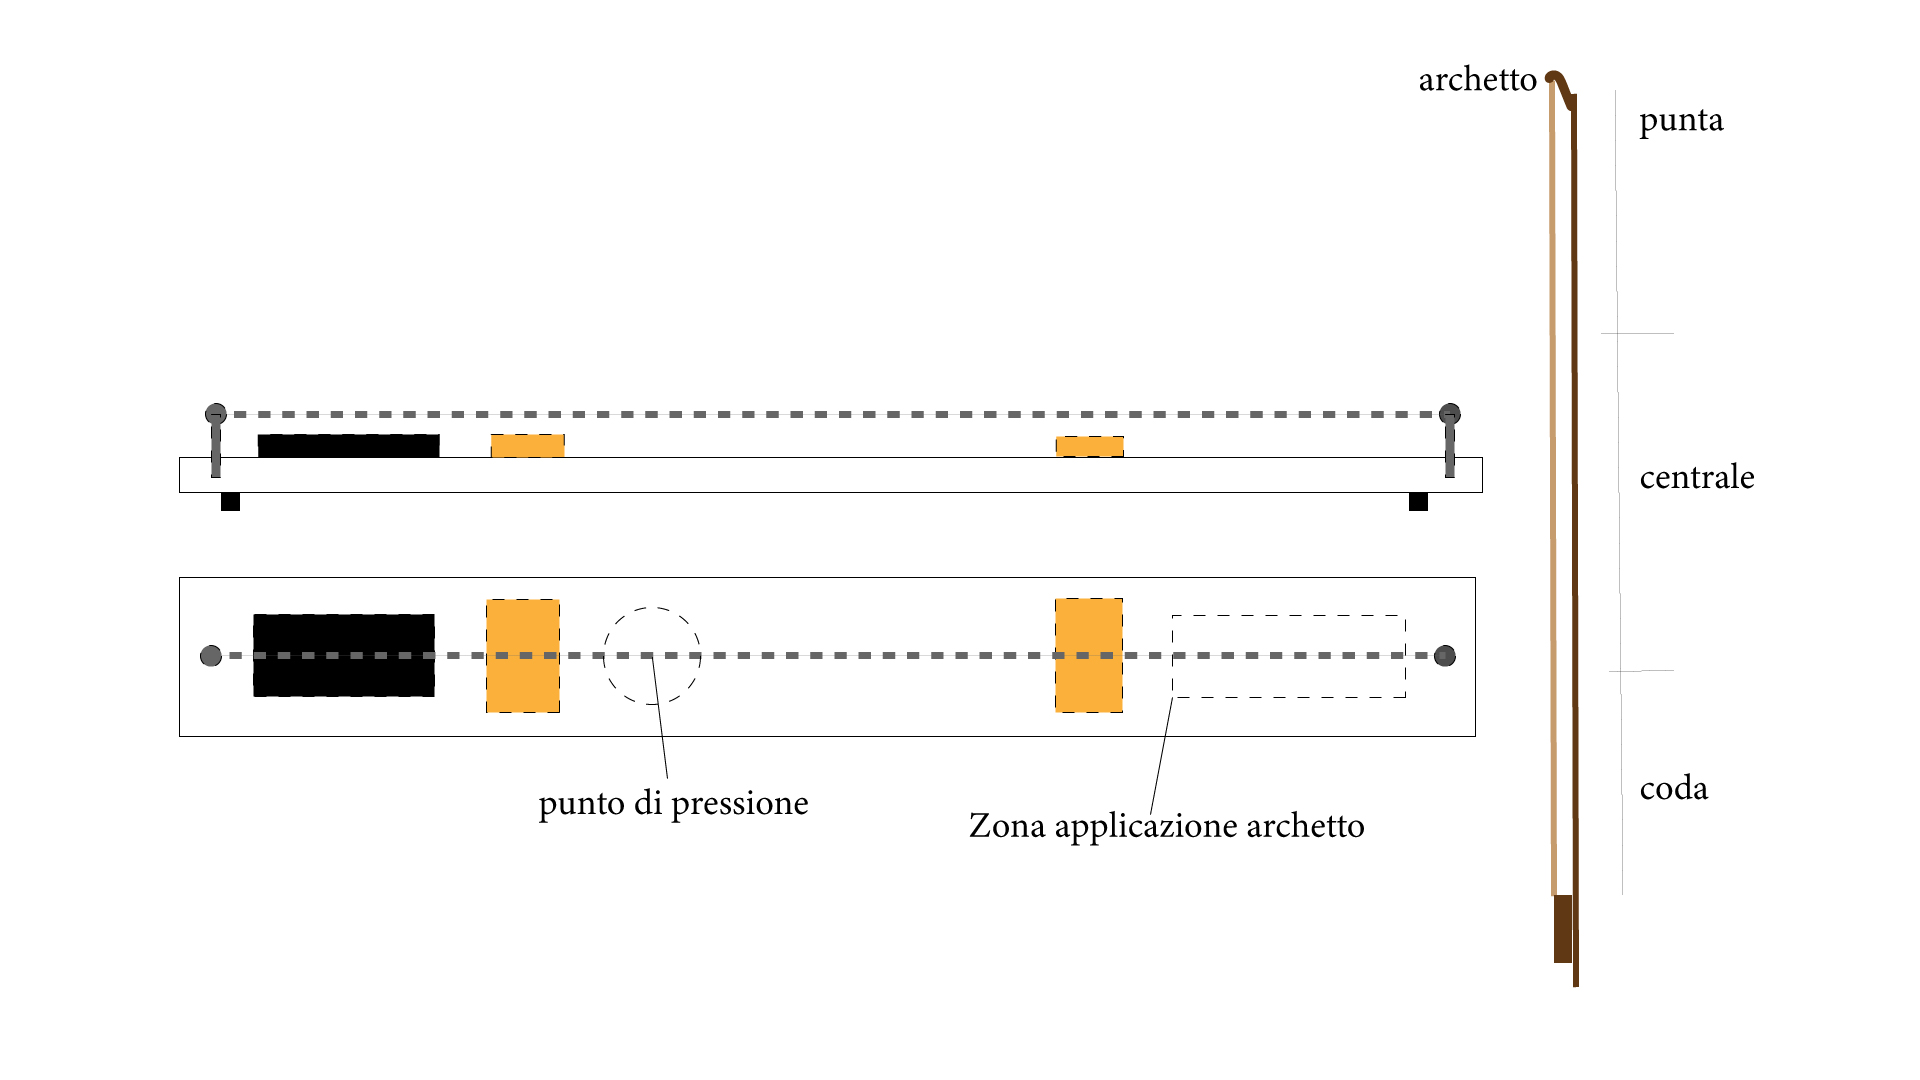
\includegraphics[width=1.\textwidth]{unamolla_schema.jpg}
\caption{Schema Unamolla 1.2}
\label{fig:03_unamolla_02}
\end{figure}

L’analisi acustica di uno strumento amplificato di nuova concezione come
\emph{Unamolla} ha molteplici gradi di variabilità legati soprattutto alla
gestualità dell’esecutore ed alla molteplicità di modalità eccitative della molla.

Non disponendo di una prassi esecutiva consolidata, è importante codificare in
modo preciso e, quanto più possibile, riproducibile, i parametri che determinano
il gesto e la modalità di eccitazione dello strumento.

Per iniziare un approccio di analisi ad Unamolla, ho deciso di utilizzare un
archetto barocco per violoncello e restringere il range di analisi a determinati
gesti.

Come si nota in figura 3, ci possiamo avvalere di vari parametri per l’analisi
di un'arcata, applicata direttamente sulla parte tratteggiata a destra.

\subsection{Tecniche di ripresa}

Tutte le riprese sono state fatte con una scheda audio e sono a $48KHz$ e $32bit$.

I campioni sono tutti mono e il segnale che otteniamo è la risultante della somma
(tramite saldatura) di:

\Large{\color{red} COME TI HO SCRITTO NELLA NOTA PRECEDENTE, TRAMITE SALDATURA NON SIGNIFICA NULLA SE C'è UNA SOMMA è TRAMITE SOMMA ANALOGICA DIRETTA, SENZA INTERVENTI DI AMPLIFICAZIONE O RIDUZIONE DEL GUADAGNO}

\begin{itemize}
  \item{Doppio Humbucker per basso}
  \item{Doppio Humbucker per chitarra}
  \item{Piezoelettrico}
\end{itemize}
\Large{\color{red} dovresti indicare le specifiche tecniche di quello che hai usato, se trovi diagrammi, nomi, codici. È una ricetta con ingredienti scelti.}

\Large{\color{red} separa la parte acustica da quella gestuale e musicale}

Di seguito diamo le definizioni dei parametri gestuali presi in considerazione
con i relativi range di valore:

\begin{description}
  \item[Archetto:] come mostrato in figura, consideriamo le tre zone punta, centrale, coda.
  \item[Angolazione archetto:] l’angolazione presa in esame è quella nell'ambito $30\sim70^\circ$.
  \item[Velocità:] lento, veloce, moderato.
  \item[Tensione:] molla libera oppure fermata con la sola pressione di uno o due dita della mano libera.
  \item[Pressione:] da 0 a 10, considerando lo zero con l’archetto semplicemente appoggiato, e il 10 come uno \textit{sf}.
\end{description}

Prendiamo in esame, un determinato gesto che ha queste caratteristiche:
\begin{description}
  \item[Zona dell’archetto:] coda
  \item[Angolatura:] $60^\circ$
  \item[Velocità:] lento
  \item[Tensione:] molla fermata che tocca la base in legno a 1/3 a destra.
  \item[Pressione:] 2
\end{description}

\Large{\color{red}Ho cambiato lo spettro, ovviamente non so se fa riferimento allo stesso campione}

In figura \ref{fig:04_spettro_01}, lo spettro in frequenza del gesto.

\begin{figure}[h]
\centering
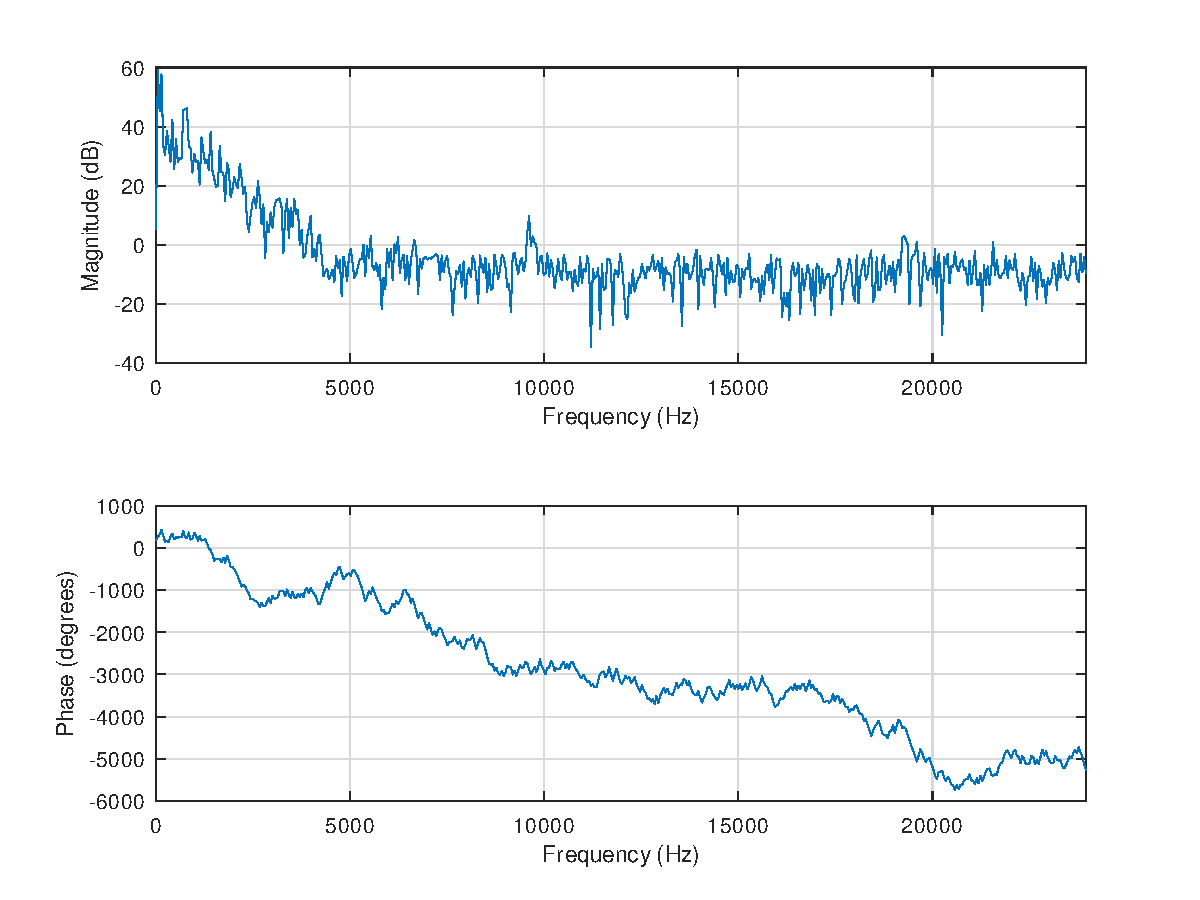
\includegraphics[width=1.\textwidth]{unamolla_octave}
\caption{Unamolla, analisi spettro}
\label{fig:04_spettro_01}
\end{figure}

Nell’esecuzione di ogni gesto emergono degli aspetti legati all’interazione
dell’esecutore con lo strumento e al feedback tattile alimentato dalla reazione
dello strumento stesso all’intervento dell’esecutore. In questo caso la reazione
più evidente è che tutto l’avambraccio e la mano avvertono una tenue modulazione
sulle basse frequenze dovuta alla vibrazione della molla sulla base di legno.
Questa vibrazione rimane fino ad una velocità moderata, con una pressione a
0.4-0.3 (in una scala da 0 a 1) e rimane fissa per tutte le zone dell’archetto,
ma va a perdersi quando la pressione e la velocità aumentano, dato che entra in
gioco un nuovo fattore che è legato sia alla vocalità dell’archetto, sia della
molla: la molla inizia a vibrare di meno sulle basse frequenze e lo strofinio
dell’arco si intensifica fino a suonare da sé.

La bassa frequenza cerchiata è quella che crea quella rugosità del suono che
possiamo apprezzare soprattutto a molla ferma con il dito e nella zona dell’archetto
vicino alla coda verso il centro. Inoltre, all’interno dello spettro sottostante
si possono identificare le punte degli inviluppi formantici. Uno a $130Hz$ e l’altro
a $750Hz$. Durante l’esecuzione di questa parte, ho notato una vocalità ben precisa
dello strumento, a circa 130 hertz (appunto) che come vediamo nello spettro
successivo, si identifica in una parziale di una curva formantica. Facendo dei
conti,

\Large{\color{red} che conti? riporta i tuoi calcoli.}

ho notato che se si considerano determinati bin che compongono la curva
formantica, si può notare come il MCD è intorno a $10\sim18Hz$, nella figura notiamo
un movimento non in banda audio a circa $18Hz$. La parte nel cerchio rosso è sui
$36Hz$, la prima delle parziali che compongono uno spettro che di base è inarmonico,
ma tramite determinati accorgimenti si può accentuare tale sua vocalità e rendere
possibile la costruzione di determinati gesti ai fini del nostro volere compositivo.
Riuscire anche a muoverci (o forse solamente a muoverci) in un universo micro-tonale.

Un altro fattore molto importante, notato durante l’esecuzione del gesto, è l’alta
variabilità di suono che avviene anche con il cambio dell’angolatura dell’arco:
a $45^\circ$ e $60^\circ$ i crini dell’archetto non si incastrano con le spire della molla.
Ovviamente può essere compositivamente interessante anche sfregare i crini
all’interno delle spire della molla, ma in quel caso abbiamo bisogno di un
archetto con poca pece, perché in quel caso la pece renderebbe difficile il
movimento dell’archetto facendo incastrare le spire con le sezioni di crini che
si vanno a formare.

Quando muoviamo l’archetto sulla molla, ci scontriamo con la pressione, che va
dosata, dato che ogni parte dell’archetto per via della tensione, suona in modo
differente, quindi a seconda della frizione e della velocità, va mosso l’archetto
in modo adeguato per creare un suono che risulti continuativo, che per gli scopi
compositivi personali è molto importante.

Venendo da una composizione come L’albe nei varchi, che precede il solo con la
molla in questo trittico, ho decisamente bisogno di un suono che sia in fase
iniziale continuativo e soggetto a micromovimenti che possano rendere il movimento
continuo non ripetitivo e che abbia realmente una direzione compositiva adeguata
al mio stile.

\textbf{Come si nota dalla seguente analisi di spettro-frequenza, dell’attacco
dell’archetto sullo strumento, ci sono due curve formantiche intorno a $100Hz$ e
a $700Hz$.}

\subsection{Considerazioni sull’amplificazione}

Ho preferito limitare il campo di ripresa agli elettromagneti e ai microfoni a
contatto, perché sono inerenti all’elaborazione del Live Electronics che andrò
ad effettuare e soprattutto sono gli unici tre canali che amplifico. Ho deciso
di unire tutte le riprese audio in un’unica uscita fisica.

Non ho notato cancellazioni fisiche del segnale. L’unione delle fonti sonore
è il risultato di varie prove effettuate per avere più dinamica ma soprattutto
più presenza dello strumento e uno spettro più ricco. La somma dei segnali è
poi il reale suono che ho ricercato per la molla.

In futuro, come esplico nello schema in figura 5, cercherò di creare una cassa
di risonanza \textbf{a lunghezza variabile} con la quale poter enfatizzare e
modificare l’amplificazione del mio strumento e non delimitare più il campo di
amplificazione al contatto, ma estenderlo ad una microfonazione differente
(tramite la cassa di risonanza ed un microfono a condensatore).

\begin{figure}[h]
\centering
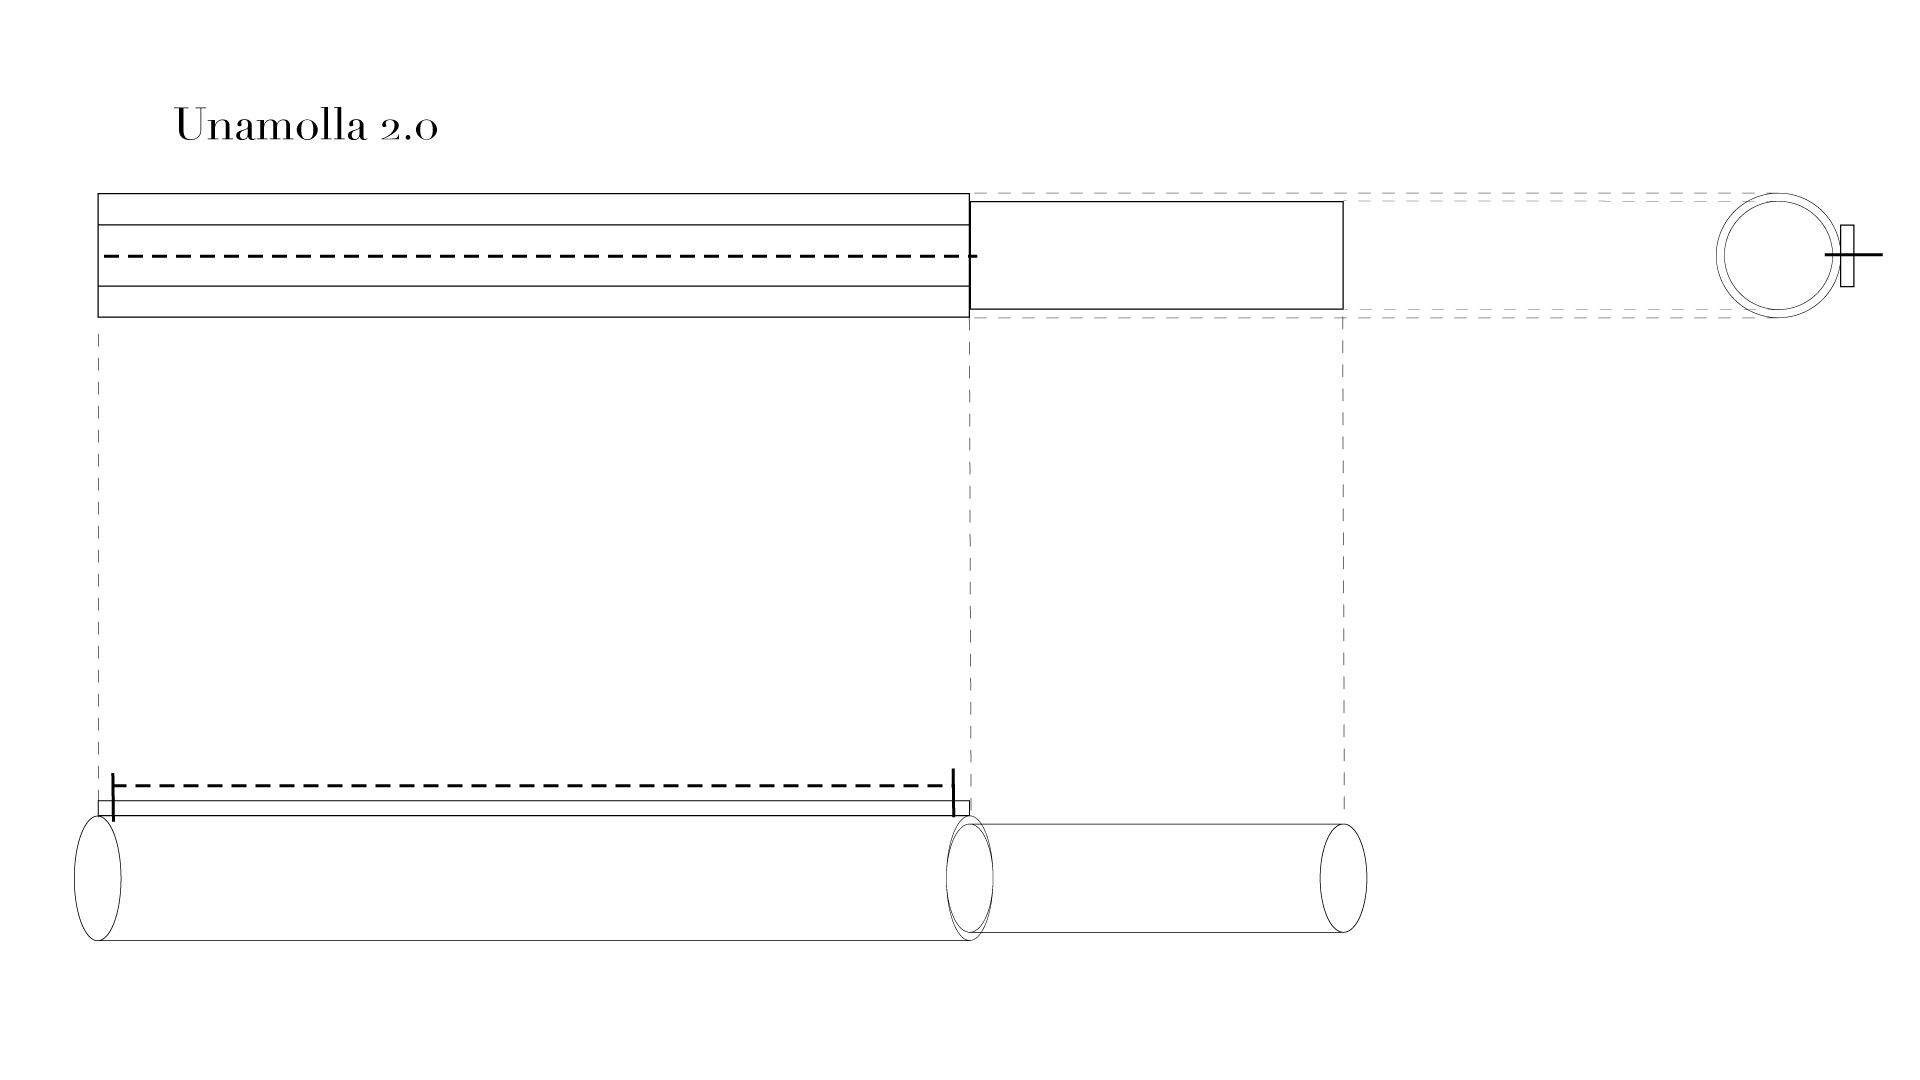
\includegraphics[width=1.\textwidth]{unamolla_2_schema.png}
\caption{Unamolla 2.0, design di Unamolla con cassa di risonanza variabile}
\label{fig:05_unamolla_2.0}
\end{figure}

\subsection{Conclusioni}

Le prime domande che mi sono poste era riguardo la comparazione con strumenti
reali e la possibilità di farli convivere all’interno di una partitura.

Per quanto riguarda lo \emph{Sp.I.R.E.} ho intrapreso uno studio gestuale molto legato
al mondo percussivo. Nel caso di Unamolla, ho deciso di avvicinarmi più al mondo
degli archi e l’analisi gestuale inizia con l’utilizzo di un archetto barocco
per violoncello. I parametri in gioco sono diversi, l’idea di trovare una
vocalità nello strumento sta appunto nella convivenza di vari fattori.

L’archetto è stato posizionato al margine sinistro della molla. La molla è stata
“fermata” con un dito creando una sorta di nodo a 1/3  dal margine destro, subito
dopo il primo humbucker per chitarra da destra. Abbiamo tre parametri che entrano
in gioco, in base ai quali è stata fatta la classificazione del gesto sono i
seguenti, legate a determinati parti della molla sulla quale avviene la speculazione.

\begin{description}
  \item[Velocità:] dato che parliamo di uno strumento pluri-amplificato,
    si nota subito, al tocco, che tra lento e moderato può rientrare un universo di
    micro velocità che scaturiscono interessanti spunti di ricerca.
		\item[Tensione:] molla libera, fermata con la sola pressione di uno o due dita
		della mano libera dell’archetto. Questa seconda tipologia di tensione ha come
		risultato l’eliminazione delle \textit{auto-vibrazioni} indotte alla molla e
		la possibilità quasi di “intonarla”. Inoltre si può fermare la molla anche
		facendole toccare la base in legno sempre pigiando con un dito nella parte
		centrale; il risultato sarà una frequenza più alta della precedente e pari
		quasi al doppio della frequenza precedente: $130Hz$. Questo comporta un indice
		di vibrazione sulle basse frequenze della molla, che diminuisce (o addirittura
		quasi scompare) quando viene fermata.
		\item[Zona dell’archetto:] Come per la velocità, queste parti contengono un
		mondo di microgesti che se uniti anche a velocità e modifiche della tensione,
		riescono a trasformare minimamente il suono inarmonico, riuscendo (anche
		tramite un’elaborazione) a eccitare la molla a tal punto da riuscire a
		sottolineare una vocalità intrinseca dello strumento.
		\item[Pressione:] ultimo ma non meno importante parametro, rende possibile
		il cambio timbrico della molla ed entrano in gioco parti inerenti all’archetto
		stesso e ad armoniche che possono venir fuori nel momento in cui si uniscono
		vari fattori, tra cui una determinata posizione dell’archetto, la velocità e
		la pressione. Ho adottato una scala da 0 a 1, dove 0.01 ad esempio è
		l’archetto in movimento semplicemente poggiato, e 1 è uno sf. Bisogna avere
		molta cura nella pressione dell’arco, perché al minimo sbaglio suona l’arco
		stesso, quasi a parere un armonico, e dirige l’attenzione dell’ascoltatore
		verso frequenze molto acute, tralasciando le medio basse che perdono di
		intensità.
\end{description}

\textbf{Tutti questi fattori possono essere riportati in partitura per precisare
a quale suono si vuole puntare tramite un determinato gesto.}

\textit{Nella difficoltà esecutiva di uno strumento con uno spettro complesso
come quello della molla, possiamo sentire risuonare vari strumenti, come trombe,
corde di contrabbasso e anche una minima vocalità se si vanno ad enfatizzare
delle parti specifiche dello spettro.}



%************************************************

\section{Catalogazione degli strumenti, gesto-segno}

Per avvicinare al mondo degli strumenti musicali di liuteria classica, lo strumento
Unamolla, ho deciso di intervallare la performance-solo dello strumento, con due
composizioni: una per sassofono soprano tape ed elaborazione; un duo per
strumento e sassofono tenore. Prima di iniziare la scrittura del duo, ho deciso
di stabilire dei parametri sui quali lavorare, delle parti simili a livello
spettrale tra i due strumenti. In primo luogo ho pensato ai multifonici e in
seguito, nella parte del duo, alla quantità di rumore indotta nello strumento
tramite un soffio più deciso nell'insufflazione  con cambiamenti della posizione
del labbro inferiore.

La catalogazione che segue, è stata ideata per riuscire ad individuare gesti
simili tra questi due strumenti di famiglie differenti: una appartenente all’universo
temperato, l’altra, al contrario, appartenente all’universo della molla, in teoria
più vicina a quello dei rumori.

Insieme ad un violista abbiamo riscontrato che ci sono varie parziali all’interno
dello spettro della molla, come si può riscontrare anche nell’analisi. C’è una
nota principale che è il LA, ma attorno, nello spettro della molla si possono
definire sia un Si che un Sol diesis crescente che un La un’ottava superiore e
un Sib.

Esistono varie aree di studio con le quali possiamo lavorare per avere un approccio
reale all’unione di strumenti occidentali e strumenti di nuova creazione:

\begin{description}
  \item[gestuale:] come detto in precedenza, studio legato al gesto fisico e
	successivamente alla creazione di un segno o simbolo che, ben spiegato in
	legenda, rende possibile l’esecuzione di una determinata cellula musicale;
  \item[comparativa:] strumenti reali in comparazione agli strumenti di nuova
	creazione;
  \item[compositivo:] unione ritmico-melodica su base formale e timbrica.
\end{description}

A livello umanistico si stanno facendo ad oggi delle indagini riguardo il gesto.
Non più una visione solo temporale dell’utilizzo di varie tecniche, ma anche
spettrale e spaziale. Lo strumento d’analisi è, quindi, nel dominio congiunto
di tempo e frequenza. Ovvero, tramite software specifici si dà spazio ad
un’analisi che ha come base lo studio delle armoniche o delle accentuazioni a
livello frequenziale in determinati gesti fatti sullo strumento.

\subsection{Strumenti a confronto: catalogazione}

Per fare un’analisi completa delle tecniche ho voluto stilare una serie di
tecniche e gesti uguali per ogni strumento che vado ad analizzare. E’ ovvio che
l’utilizzo delle chiavi è strettamente legato al flauto, ma a mio parere
documentare tutte le tecniche rende ancora più palese la possibilità di rendere
omogeneo questo studio.

\begin{table}[htp]
\caption{Sassofono Soprano, tabella comparativa tecniche}
\begin{center}
\begin{tabular}{ccc}
\hline
\textbf{Tecniche/Strumento} & \textbf{Unamolla} & \textbf{Sassofono Soprano} \\
\hline
Pizzicato & SI & NO \\
\hline
Grattato & SI & NO \\
\hline
Flautato & SI & SI \\
		&con archetto & \\
\hline
Nota lunga & SI & SI \\
		&con motore & \\
\hline
Nota corta & Mallet & SI \\
		&in metallo & \\
\hline
Trillo & NO & SI \\
\hline
Frullato & SI & SI \\
		&con motore & \\
\hline
Glissato & NO & SI \\
		& & ma solo su \\
				& & piccoli intervalli \\
\hline
Vibrato & NO & SI \\
\hline
Variazione & SI & SI \\
di quarto di tono & con motore & \\
& o archetto & \\
\hline
Variazione di tono & SI & SI \\
& solo se si crea & \\
& un nodo centrale & \\
\hline
Fruscìo & SI & SI \\
\hline
Soffio & NO & NO \\
\hline
Chiavi & NO & SI \\
\hline
Armonici & SI & SI \\
\hline
Bicordi & NO & MULTIFONICI \\
\hline
Tricordi & NO & MULTIFONICI \\
\hline
Accordi & NO &NO \\
\hline
\end{tabular}
\end{center}
\label{default}
\end{table}%

Come possiamo vedere dalla prima tabella, alcune tecniche che sono di natura come
per uno strumento come il SASSOFONO SOPRANO, diventano un po’ più complessi da
riprodurre per la molla. Ad esempio il frullato non può essere riprodotto, ma
può venire eseguito dalla molla tramite un motorino continuo (vibratore o rasoio
per capelli). Ho voluto anche specificare la presenza o meno dell’archetto con
la molla per poter scrivere più precisamente anche i segni inerenti alla natura
della tecnica eseguita sul nuovo strumento. Ultimo gesti presente in Unamolla è
legato al suo feedback. Tramite un overdrive della BOSS e un CRY-BABY (pedale wah-wah)
ho la possibilità di eccitare determinate armoniche della molla e di riuscire,
tramite il pedale, a controllare il feedback, riuscendo a definire dei piccoli
cambiamenti microtonali.
